\chapter{Introducción a RFID}

\section{Identificación por radiofrecuencia}

En los años recientes los sistemas de identificación por radiofrecuencia 
(RFID por sus siglas en inglés) se han vuelto muy populares en áreas como 
logística, control de acceso, industria manufacturera e incluso transporte. 
Esto es debido a que brindan información segura, actualizada y permiten 
llevar un control eficiente del estado de los productos a un muy bajo costo 
de mantenimiento.

Este tipo de sistemas forma parte de los que se conocen como sistemas de 
\emph{identificación automática} (Auto-ID), donde tal vez el de uso más 
extendido sea el código de barras. El RFID nace como una evolución natural 
dedicada a identificar o realizar el seguimiento de personas o productos, y 
que supera al código de barras en cuanto a cantidad de datos almacenables, 
no requiere línea de visión directa y permite la lectura simultánea de 
múltiples artículos. Se trata de un sistema que está directamente 
relacionado con las clásicas \emph{tarjetas inteligentes}, que eran 
dispositivos de almacenamiento electrónico de datos, con posibilidad de 
algún procesamiento que, por conveniencia, tenían el tamaño de una tarjeta 
de crédito. Sin embargo, en los sistemas de RFID la alimentación del 
dispositivo portador de información y la transmisión de datos no se realiza 
utilizando contacto galvánico sino que se realiza utilizando campos 
magnéticos o electromagnéticos y por lo tanto se evitan los problemas de 
desgaste y el consecuente mantenimiento asociado. Se trata entonces de un 
sistema de identificación inalámbrica rápido y robusto.

Un sistema de identificación por radiofrecuencia está formado por un \emph
{interrogador} o \emph{lector} y uno o varios \emph{transponders}, que 
generalmente toman la forma de tarjetas personales y/o etiquetas 
autoadhesivas (RFID \emph{tags}). Cada transponder cumple el rol de portador 
de información tal como un número de identificación, datos de un producto o 
saldo restante si se trata de un pasaje electrónico. Debido a su reducido 
tamaño y peso son dispositivos ideales para ser transportados por personas y 
animales, o para ser adheridos a envases. Normalmente están formados por un 
dispositivo de acoplamiento, que permite realizar el vínculo con el lector a 
través de campos magnéticos o electromagnéticos, y un circuito integrado que 
se encarga de almacenar y procesar la información e implementa un protocolo 
de comunicación para transmitir esa información sin pérdida de datos. Es al 
diseño del circuito integrado que estará dedicado gran parte del presente 
trabajo de tesis.

\begin{figure}
	\centering
	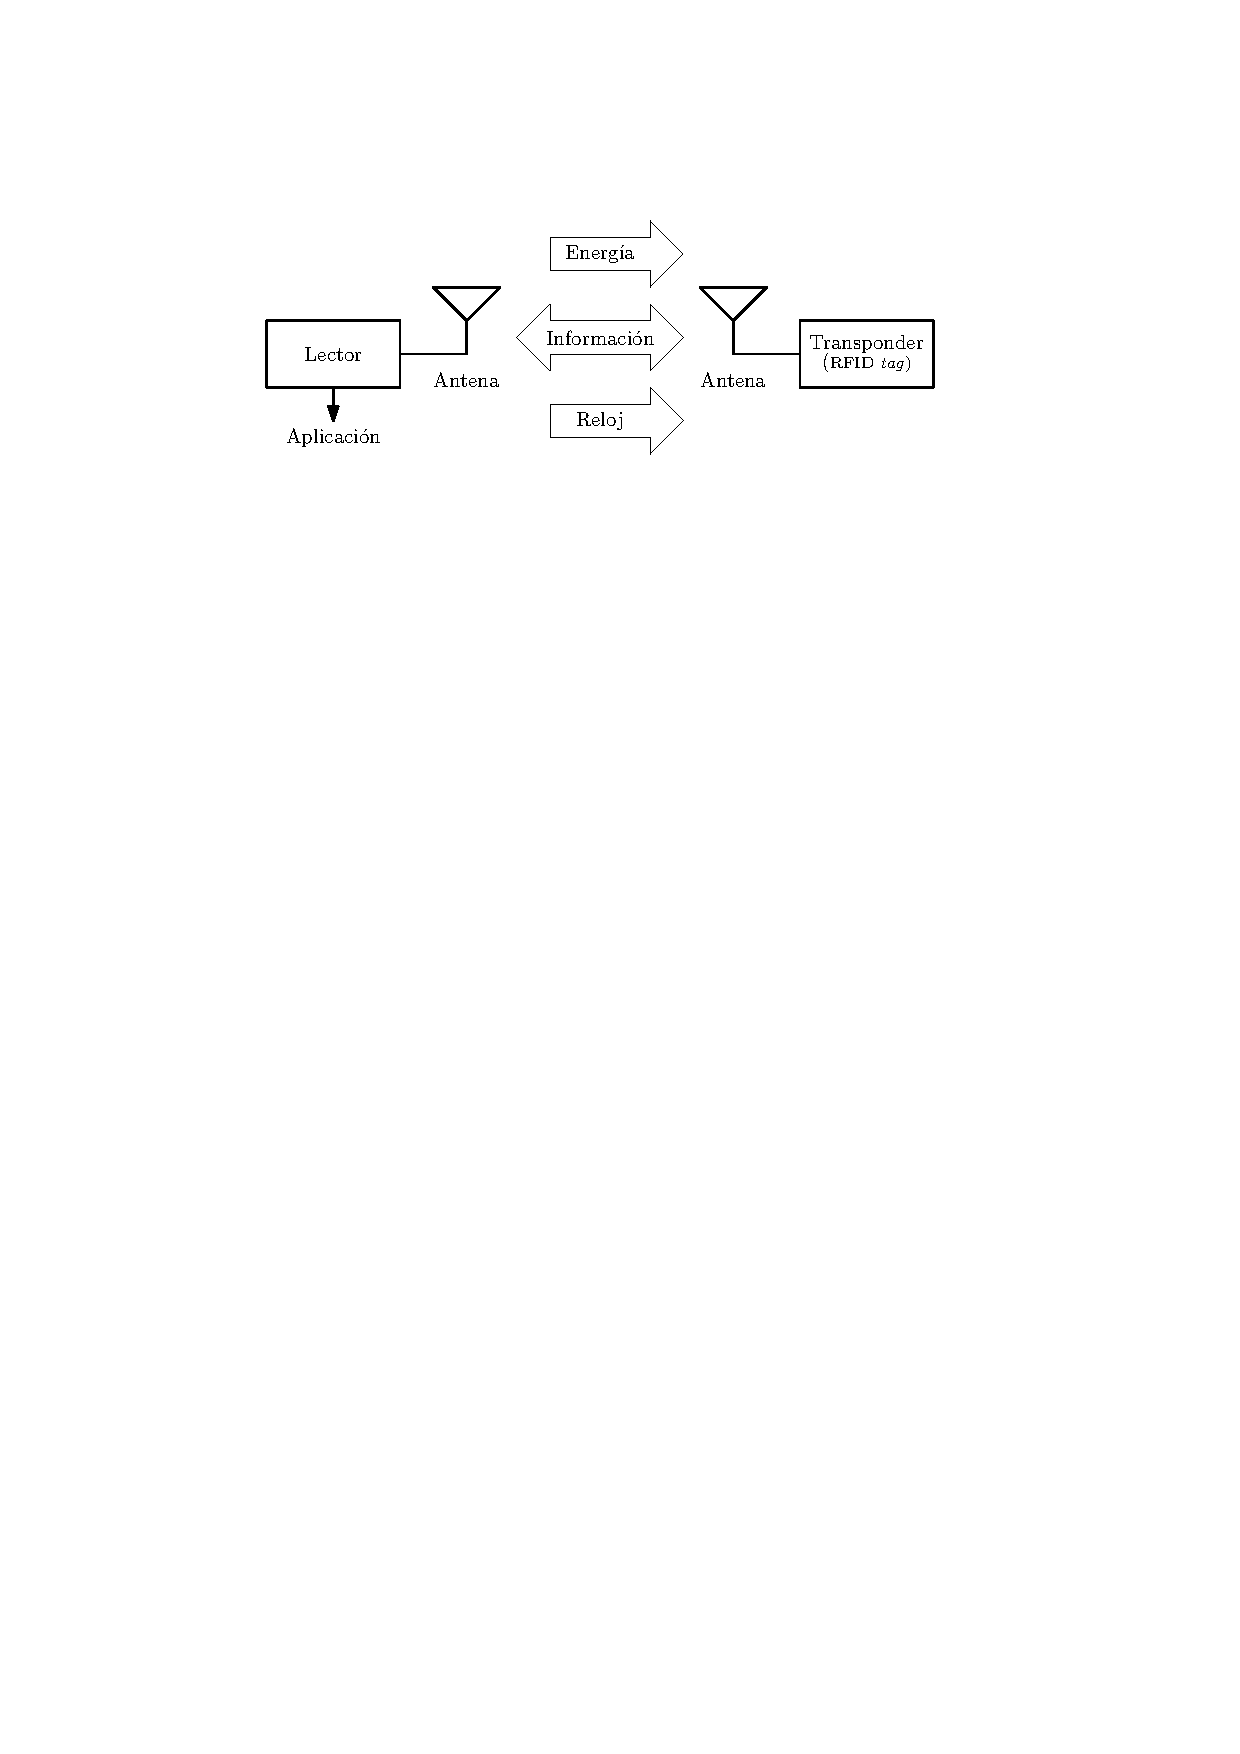
\includegraphics{SistemaRFID}
	\caption{Esquema típico de un sistema de identificación por radio 
	frecuencia. Lector y transponder son los componentes principales.}
	\label{fig:SistemaRFID}
\end{figure}

La comunicación con el transponder se realiza a través de campos magnéticos 
o electromagnéticos que, dependiendo de la tecnología utilizada, se 
encuentran en las bandas de LF (Low Frequency), HF (High Frequency) o UHF (Ultra High Frequency). El lector cuenta con una antena 
con la que mantiene el campo dentro de su área de influencia. Cuando un 
transponder ingresa dentro del campo generado por el lector, por un lado se 
transmite energía desde el lector hacia el transponder, que en el caso de un 
tag pasivo será utilizada para alimentar los circuitos internos; y por otro 
se produce un vínculo entre el lector y el transponder que puede ser 
utilizado para transmitir información. En general la información se envía 
realizando algún tipo de modulación sobre el campo. Al ser el lector la 
fuente del campo electromagnético, es muy común interrogar al transponder 
modulando la amplitud y/o fase, mientras que para transmitir información en 
sentido inverso, desde el transponder hacia el lector, se utiliza modulación 
de carga o variaciones en el coeficiente de reflexión.

\section{Clasificación de los sistemas de RFID}

Existen numerosos sistemas de identificación por radio frecuencia, casi 
tantos como fabricantes, por lo que se debe realizar algún tipo de 
clasificación que permita entender el alcance del presente trabajo. Además, 
tener una clasificación permite reducir esa gran variedad a algunas pocas 
categorías con las que se pueden reconocer las características principales 
de cada sistema. Por ejemplo, algunas características que pueden 
interesarnos son: la \emph{distancia de operación} que está relacionada con 
parámetros como frecuencia y potencia; la longitud de \emph{penetración} de 
las ondas, para saber si el dispositivo puede ser interrogado dentro de la 
piel o debajo del agua y que también está relacionada con la frecuencia; 
velocidad de transmisión de datos, etc\...

La frecuencia de operación se encuentra en un amplio rango del espectro 
electromagnético ya que existen sistemas que operan desde onda larga a \SI
{135}{\kilo\hertz} hasta microondas a \SI{5.8}{\giga\hertz}. El acoplamiento 
físico se realiza utilizando campos \emph{eléctricos}, \emph{magnéticos} o 
\emph{electromagnéticos} y el alcance típico de los sistemas varía de 
algunos milímetros a decenas de metros.

Los transponders pueden ser activos o pasivos, según la forma en 
la que obtienen la energía. Se dice que un transponder es \emph{activo} 
cuando cuenta con energía propia (se alimenta a través de pilas o baterías), 
lo que generalmente se utiliza para lograr un alcance mayor. Por otra parte 
se les dice \emph{pasivos} a aquellos que no cuentan con energía propia y 
por lo tanto dependen de la energía proporcionada por el lector para 
funcionar. Estos últimos son los más difundidos en el mercado ya que al no 
contar con baterías su costo se reduce drásticamente respecto de los activos.

Los sistemas de RFID de muy corto alcance, menos de \SI{1}{\cm}, se conocen 
como <<\emph{sistemas de acoplamiento cercano}>> (\emph{close-coupling 
systems}). La lectura del transponder se realiza insertándolo en el lector o 
bien posicionándolo sobre una superficie dispuesta para tal fin. Los 
sistemas de acoplamiento cercano utilizan campos eléctricos o magnéticos y 
teóricamente pueden funcionar desde cero hasta \SI{30}{\mega\hertz}, ya que 
no dependen del fenómeno de radiación. El gran acople existente en este tipo 
de sistemas facilita la transmisión de energía y por lo tanto pueden 
utilizarse grandes cargas e incluso microprocesadores con consumos de potencia no 
optimizados. Estos sistemas se utilizan principalmente en aplicaciones donde 
se requiere una estricta seguridad y que a su vez no es necesario un largo 
alcance, como por ejemplo cerraduras electrónicas o sistemas electrónicos de 
pago.

Los sistemas con un alcance de hasta \SI{1}{\meter} se conocen como <<\emph
{sistemas de acoplamiento remoto}>> (\emph{remote coupling systems}). Casi 
todos estos sistemas están basados en \emph{acoplamiento inductivo}, es 
decir, utilizan campos magnéticos para establecer el enlace entre el lector 
y el transponder. El acoplamiento inductivo se utiliza hoy en día en por lo 
menos el 90\% del mercado de RFID y es por ese motivo que se le prestará 
especial importancia a lo largo del informe. Trabajan a frecuencias de \SI
{135}{\kilo\hertz}, \SI{13.56}{\mega\hertz} y en algunas aplicaciones 
especiales a \SI{27.125}{\mega\hertz}.

Los sistemas de RFID con un alcance mayor a \SI{1}{\meter} se conocen como <<
\emph{sistemas de largo alcance}>> (\emph{long-range systems}). Todos los 
sistemas de largo alcance utilizan ondas electromagnéticas en las bandas de 
UHF y microondas, con frecuencias desde \SI{868}{\mega\hertz} hasta \SI{5.8}{
\giga\hertz}. Los transponders trabajan de un modo parecido a un radar 
produciendo la reflexión de las ondas emitidas por el lector para 
comunicarse. Utilizando tags pasivos es común lograr un alcance de 
aproximadamente \SI{3}{\meter}, mientras que con tags activos es posible 
alcanzar los \SI{15}{\meter} o más. Sin embargo, la energía proveniente de 
la batería en los tags activos no se utiliza para realizar la transmisión de 
datos, sino que es utilizada solo para alimentar los circuitos internos de 
procesamiento y retención de datos. La única energía utilizada para 
transmitir información es la proveniente del mismo lector a través del campo 
electromagnético.

\section{Estandarización de los sistemas de RFID}

La estandarización es un tema crítico en los sistemas de identificación, ya 
que permite la interoperabilidad entre distintas empresas y sectores. Un 
sistema estándar puede ser utilizado por toda la cadena de suministro de un 
producto y de esta forma se pueden identificar los ítems que la transitan de 
manera unívoca.

A través de los años se han definido numerosos documentos, como por ejemplo: 
ISO 11784/5 para la identificación de animales, ISO/IEC 14443 para tarjetas 
de identificación por proximidad (Proximity cards), ISO/IEC 15961/2 para la 
administración de productos, ISO/IEC 15693 para tarjetas de identificación 
por cercanía (Vicinity cards), ISO/IEC 18000 para el seguimiento de 
productos, etc. Dentro de las normas mencionadas, la ISO/IEC 14443 a tomado 
especial relevancia debido a que numerosos medios de pago electrónico se 
basan en ella para acceder al medio y luego trabajan con protocolos 
propietarios de nivel superior, como es el caso de las tarjetas MiFare de 
NXP. 

El estándar ISO/IEC 14443 está dividido en cuatro partes en las que se 
definen las características físicas de las tarjetas en cuanto a tamaño y 
forma; frecuencia de operación, símbolos y características de señal (la capa 
física del protocolo); luego se definen tamaños y características de las 
tramas, un método para evitar colisiones y que permite seleccionar uno de 
entre varios transponders dentro del alcance del lector; y por último define 
un protocolo de alto nivel, de carácter opcional, para transmitir 
información e intercambiar mensajes de control y de estado.

En el estándar ISO/IEC 14443 se trabaja con campos magnéticos variables en 
la banda libre para uso industrial, médico y científico (ISM) a una 
frecuencia de 13,56MHz (HF), y el transponder utiliza un inductor de tamaño 
no mayor al de una tarjeta ID--1 \cite{ISO7810} 
para establecer el enlace con el lector. Se 
trata de un acoplamiento inductivo débil ya que el campo magnético se 
encuentra disperso en el espacio, al contrario de lo que ocurre en un 
transformador.

A continuación se realizará una breve reseña del contenido de cada parte de 
la norma. Las partes 2 y 3 contienen la información acerca de las señales, 
símbolos y codificaciones utilizadas en el sistema y por lo tanto se les 
prestará especial atención. La parte 4 se dejará de lado ya que, además de 
ser opcional, define un protocolo de alto nivel con paquetes de datos que no 
será implementado.

% \todo{Relacionar el estándar con el modelo OSI (RFID Handbook, pág 257) y 
% explicar por que se le prestar más atención a la parte 2}

\subsection{ISO/IEC 14443 -- Parte 1: Características físicas}

En la primera parte del documento se realizan dos definiciones importantes 
que serán utilizadas luego a lo largo de toda la norma.

\begin{itemize}
	\item{Se define al transponder, el dispositivo portador de la 
	información, como PICC: <<\emph{Proximity Integrated Circuit Card}>>}
	
	\item{Se define al lector, que es el dispositivo que produce el campo 
	magnético y se comunica con el transponder a través de acoplamiento 
	inductivo, como PCD: <<\emph{Proximity Coupling Device}>>}
\end{itemize}

También se definen las características físicas del transponder en cuanto a 
tamaño y forma. Se limita el tamaño de la antena a \SI[product-units = 
brackets]{86 x 54 x 3}{\milli\meter} ya que la interfaz de radiofrecuencia y 
los bancos de prueba, que están definidos en la norma ISO/IEC 10373--6 \cite
{ISO10373Part6}, son para una antena del tamaño de una tarjeta tipo ID--1. 
El estándar ISO/IEC 7810 define el tamaño de este tipo de tarjetas.

Además se incluye información acerca de la radiación ultravioleta, rayos~X, 
campos eléctricos y magnéticos, y temperaturas máximas que deben soportar 
las tarjetas.

\subsection{ISO/IEC 14443 -- Parte 2: Interfaz de radiofrecuencia para señal 
y energía}
\label{sec:ISO14443_2}

En esta segunda parte se describe el método utilizado para transferir la 
energía desde el PCD (lector) hacia la PICC (tarjeta). El PCD debe generar 
un campo magnético alterno a una frecuencia de \SI{13.56}{\mega\hertz} \(\pm
\) \SI{7}{\kilo\hertz} y las PICC deben acoplar inductivamente ese campo 
para recibir energía, y modularlo para transmitir información. La frecuencia 
de trabajo del sistema se define como \(f_c = \SI{13.56}{\mega\hertz}\). 
Prácticamente todos los parámetros se definen luego en función de \(f_c\), 
por lo que se convierte en un valor extremadamente importante para el diseño.

Luego se definen los valores máximos y mínimos de campo magnético que el PCD 
debe ser capaz producir dentro de su volumen de operación, y con los que las 
PICC deben funcionar correctamente. Los valores pueden verse en la tabla \ref
{tab:NivelesDeCampo}.

\begin{table}
	\centering
	\begin{tabu} to 0.6\textwidth {X[c]X[c]}
		\toprule
		\multicolumn{2}{c}{Intensidad de campo magnético \si[per-mode=symbol]
		{[\ampere\per\meter]_{rms}}} \\
		\midrule
		\rowfont[c]{} \(H_{\text{mín}}\) & \(H_{\text{máx}}\) \\
		\rowfont[c]{} \(1.5\) & \(7.5\) \\
		\bottomrule
	\end{tabu}
	\caption{Límites para la intensidad del campo magnético dentro de los 
	cuales deben operar las PICC, y que no deben ser superados por el PCD.}
	\label{tab:NivelesDeCampo}
\end{table}

La comunicación con el transponder se realiza siguiendo una lógica \emph
{maestro--esclavo}, donde el PCD tiene el rol de dispositivo maestro y es el 
encargado de encuestar periódicamente a los transponders; mientras que las 
PICC hacen de dispositivos esclavos, esperando en silencio a recibir un 
comando para transmitir sólo su respuesta.

La transmisión de información desde el PCD hacia la PICC se realiza a través 
de la modulación de amplitud del campo magnético, mientras que la 
transmisión en sentido inverso, desde la PICC hacia el PCD, se realiza 
conectando y desconectando una carga que toma energía del campo magnético 
(Modulación de carga). La conexión y desconexión se realizan al ritmo de una 
subportadora que se encuentra modulada por la información transmitida.

Se definen dos interfaces de comunicación: Tipo A y Tipo B. Cada interfaz 
define su propio protocolo, que cuenta con una serie de símbolos y comandos. 
El PCD debe ser compatible con ambas interfaces y debe alternar entre ellas 
mientras se encuentra en reposo, antes de detectar la presencia de una 
tarjeta. Las PICC implementan solo una de las interfaces, ya sea tipo A o 
tipo B. Una vez establecida la comunicación se utiliza la interfaz 
correspondiente a ese transponder hasta su finalización. En la figura \ref
{fig:TransmisionTipoA_B} se muestran ejemplos de comunicación con cada una 
de las interfaces. 

\begin{figure}
	\centering
	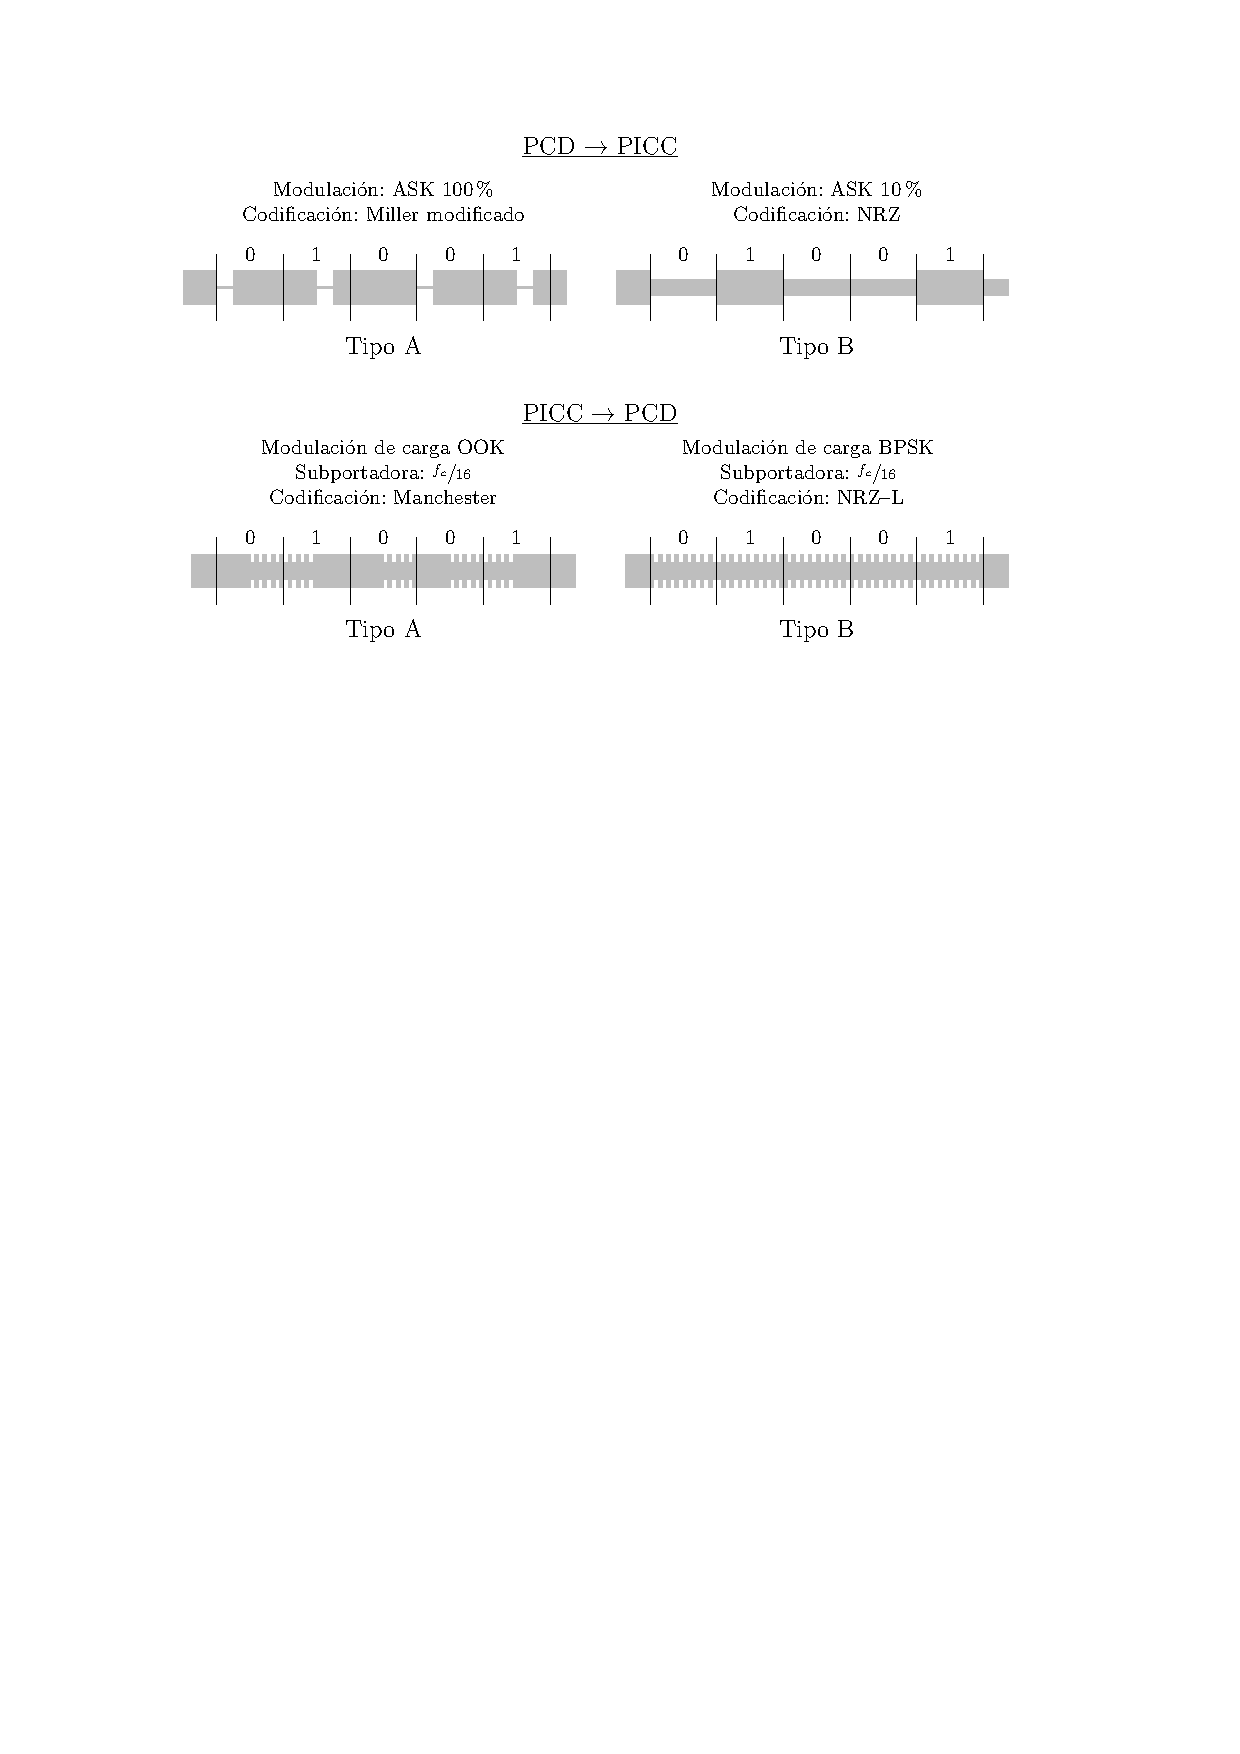
\includegraphics[width=\textwidth]{TransmisionTipoA_B}
	\caption{Ejemplos de transmisión desde el PCD hacia la PICC y viceversa, 
	para las interfaces tipo A y B a una tasa de \(\sfrac{f_c}{128}\) bits 
	por segundo (\(\sim\)\SI[per-mode=symbol]{106}{\kilo\bit\per\second}).}
	\label{fig:TransmisionTipoA_B}
\end{figure}

La tasa de transmisión de bits <<\emph{bit rate}>> se definió inicialmente 
como \(\sfrac{f_c}{128}\) \si[per-mode=symbol]{\bit\per\second}, lo que 
equivale a aproximadamente \SI[per-mode=symbol]{106}{\kilo\bit\per\second}. 
Sin embargo a medida que pasaron los años y se fue mejorando la tecnología 
también se fueron agregando al estándar velocidades cada vez más altas con 
carácter opcional y que se negocian entre los dispositivos al momento de 
establecer el enlace. Así, además de \(\sfrac{f_c}{128}\) \si
[per-mode=symbol]{\bit\per\second} se tiene \(\sfrac{f_c}{64}\), \(
\sfrac{f_c}{32}\) y \(\sfrac{f_c}{16}\) \si[per-mode=symbol]{\bit\per\second
}. La tasa de transmisión original es obligatoria para cumplir con el 
estándar y se utiliza durante las etapas de inicialización y anticolisión. 

El circuito integrado a diseñar será 
compatible con la interfaz tipo A a una tasa de \(\sfrac{f_c}{128}\) \si
[per-mode=symbol]{\bit\per\second} debido a que históricamente gran parte 
del mercado de RFID se decidió por esa interfaz y velocidad. Entonces, para 
no extender demasiado la descripción del estándar y evitar la confusión 
entre interfaces, a continuación se mencionarán solo las secciones de la 
norma relacionadas con la interfaz tipo A a la tasa de transmisión original 
de la norma.

\bigskip
El envío de información desde el PCD hacia la PICC según la 
interfaz tipo A a \(\sfrac{f_c}{128}\) \si[per-mode=symbol]{\bit\per\second} 
se realiza modulando la amplitud del campo magnético con un índice de 
modulación del 100\% (\emph{Amplitude--shift Keying 100\%}), lo que produce 
que la señal de RF se extinga durante cierto tiempo. A esa pausa que se 
produce en el campo magnético se la llama <<PauseA>>. La norma define los 
tiempos de crecimiento y decrecimiento de la señal de RF, la amplitud máxima 
en la zona de 100\% de modulación y el sobre pico máximo que puede existir 
al retornar la señal a su nivel de operación \cite[pág.~7]{ISO14443Part2}. 
La duración de la pausa se define dando valores máximos y mínimos dentro de 
los cuales deben operar los dispositivos para cumplir la norma. El valor 
típico de duración puede tomarse como \(\sfrac{32}{f_c}\) segundos (\(
\sim\SI{2.36}{\micro\second}\)).

Para la codificación de la información transmitida desde el PCD hacia la 
PICC se definen tres tipos de secuencias \cite[pág.~14]{ISO14443Part2}:

\begin{itemize}
	\item{
		Secuencia X: Se envía una \emph{PauseA} luego de un tiempo (\(t_x\)) 
		igual a la mitad de la duración de un bit.
	}
	
	\item{
		Secuencia Y: No se modula la señal durante el tiempo total del bit 
		(\(t_b\))
	}
	
	\item{
		Secuencia Z: Se envía una \emph{PauseA} al comienzo del tiempo del bit.
	}
\end{itemize}

Operando a \(\sfrac{f_c}{128}\) \si[per-mode=symbol]{\bit\per\second} el 
tiempo de duración del bit \(t_b\) queda definido como \(\sfrac{128}{f_c}\) 
segundos (\(\sim\SI{9.44}{\micro\second}\)), mientras que la mitad de 
duración \(t_x\) es \(\sfrac{64}{f_c}\). En la figura \ref
{fig:SecuenciasPCD_PICC} puede verse una ilustración de las secuencias X, Y 
y Z.

\begin{figure}
	\centering
	\begin{subfigure}{0.45\textwidth}
		\centering
		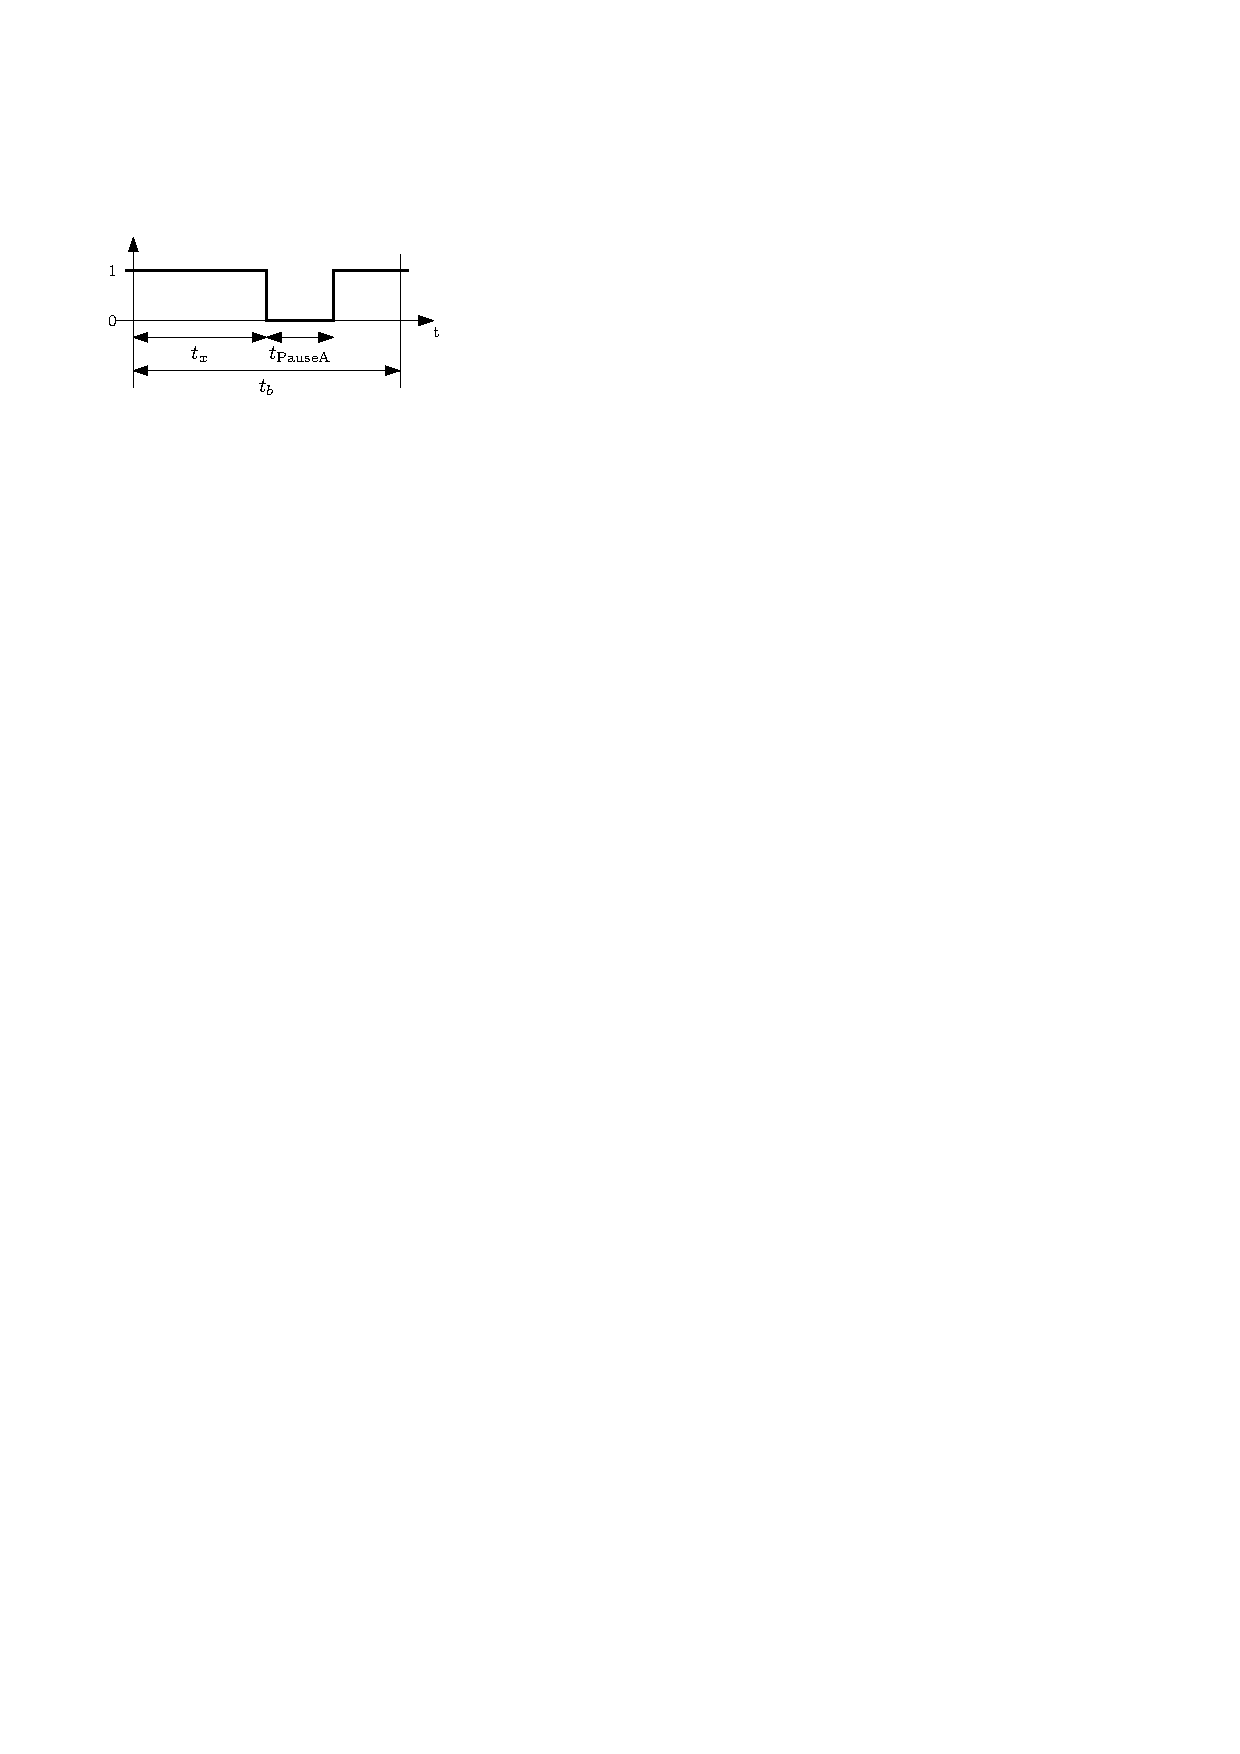
\includegraphics{SecuenciaX}
		\caption{Secuencia X.}
		\label{fig:SecuenciaX}
    \end{subfigure}%
    ~
    \begin{subfigure}{0.45\textwidth}
	    \centering
		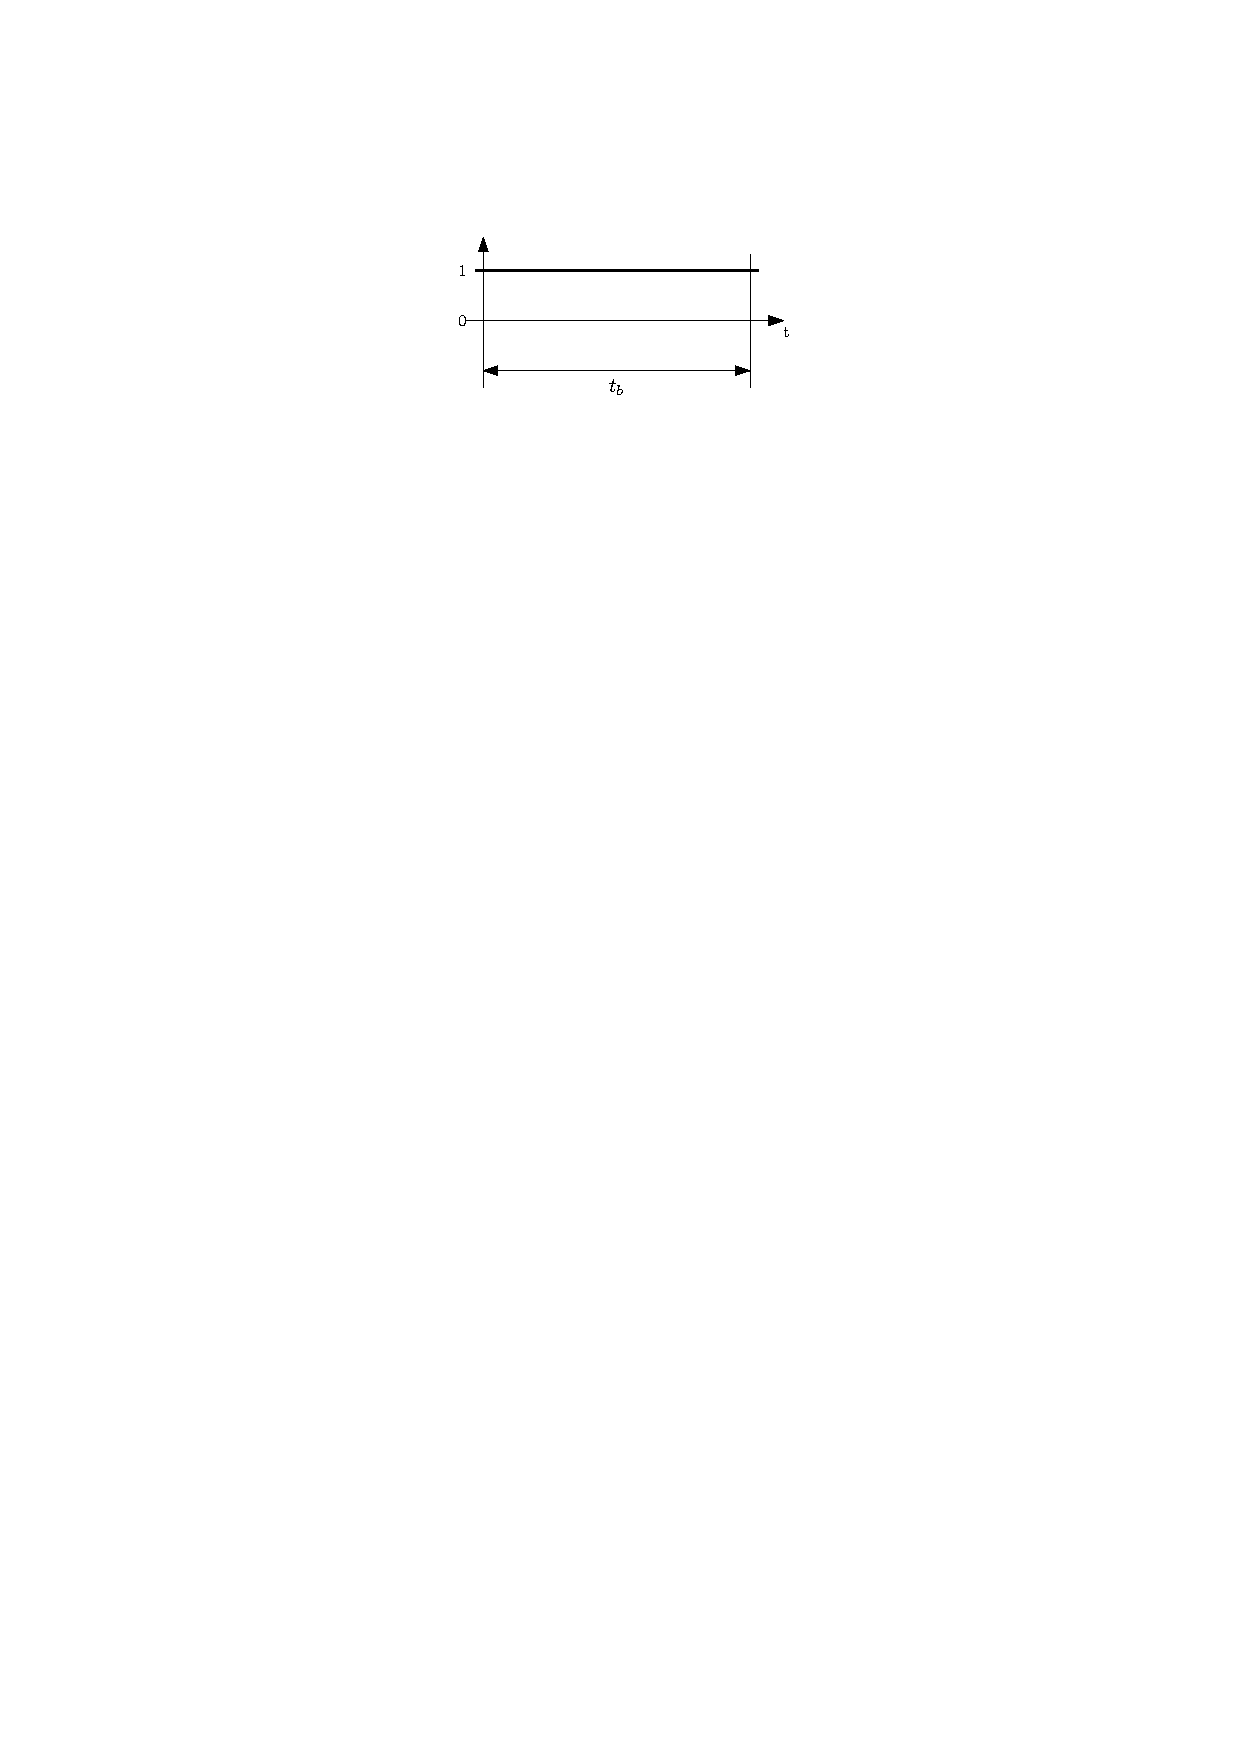
\includegraphics{SecuenciaY}
		\caption{Secuencia Y.}
		\label{fig:SecuenciaY}
    \end{subfigure}%
    \\
    \vspace{3mm}
    \begin{subfigure}{\textwidth}
		\centering
		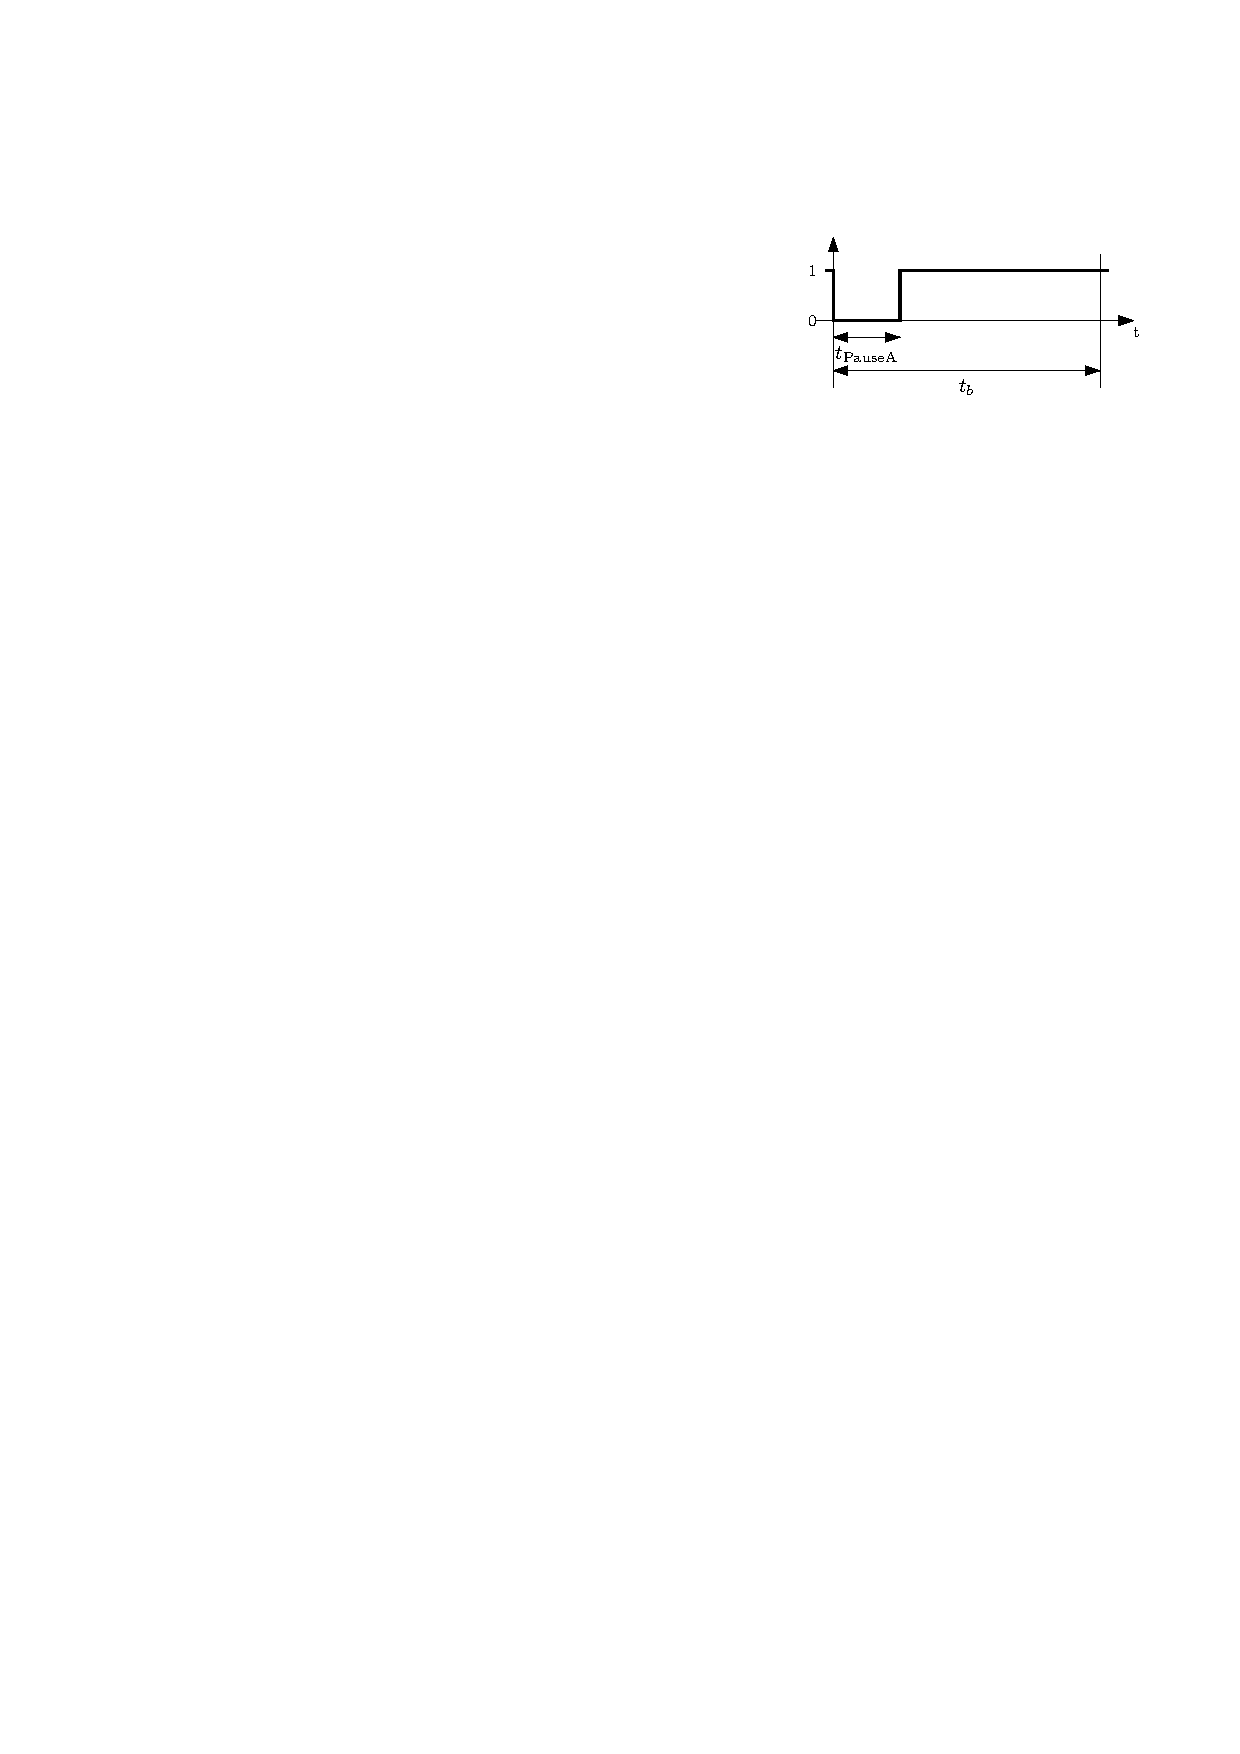
\includegraphics{SecuenciaZ}
		\caption{Secuencia Z.}
		\label{fig:SecuenciaZ}
    \end{subfigure}%
    
	\caption{Ilustración de las secuencias definidas por el estándar para la 
	transmisión de información desde el PCD hacia la PICC. El estado <<1>> 
	corresponde a la señal estable (sin modular) y el estado <<0>> a la 
	señal modulada. \(t_x = \sfrac{64}{f_c}\), \(t_{\mathrm{PauseA}} = 
	\sfrac{32}{f_c}\) y \(t_b = \sfrac{128}{f_c}\).}
	
	\label{fig:SecuenciasPCD_PICC}
\end{figure}

Con las secuencias anteriores el estándar define los símbolos utilizados en 
la comunicación, que pueden verse en la tabla \ref
{tab:CodificacionPCD_PICC}. Cada símbolo se encuentra definido según el 
orden temporal de las secuencias X, Y y Z. Por ejemplo, cuando el PCD envía 
un cero lógico debe saber si la secuencia anterior fue Y, en cuyo caso 
enviará Z, o, si fue X, deberá enviar Y. Por lo tanto el lector debe contar 
con cierta memoria a la hora de codificar los símbolos. Lo mismo ocurre en 
la PICC cuando debe decodificar la trama recibida.

\begin{table}
	\centering
	\begin{tabu}{ccl}
		\toprule
		Símbolo & Secuencia previa & Representación \\
		\midrule
		<<1>>                  &               & Secuencia X    \\
		\addlinespace
		\multirow{3}{*}{<<0>>} & Secuencia X   & Secuencia Y    \\
		~                      & Secuencia Y   & Secuencia Z    \\
		~                      & Secuencia Z   & Secuencia Z    \\
		\addlinespace
		<<Inicio>>             &               & Secuencia Z    \\
		\addlinespace
		<<Fin>>                &    & <<0>> lógico seguido de una secuencia Y \\
		\addlinespace
		<<Silencio>>           &    & Al menos dos secuencias Y consecutivas \\
		\bottomrule
	\end{tabu}
	
	\caption{Definición de los símbolos utilizados en la comunicación desde 
	el lector hacia el transponder.}
	
	\label{tab:CodificacionPCD_PICC}
\end{table}

\bigskip
Como se mencionó antes, las PICC se comunican con el PCD a 
través del acople inductivo, cargando la señal portadora de frecuencia \(f_c 
= \SI{13.56}{\mega\hertz}\) con una subportdora de frecuencia \(f_s = 
\sfrac{f_c}{16}\), lo que equivale a aproximadamente \SI{848}{\kilo\hertz}, 
que a su vez es modulada por los datos a transmitir. El estándar especifica 
que la subportadora debe generarse conmutando una carga dentro del 
transponder.

La norma fija un valor mínimo de \(\sfrac{22}{\sqrt{\text{H}}}\) \si{[
\milli\volt p]} para la amplitud producida por la modulación de carga de la 
PICC, donde H es el valor eficaz de la intensidad del campo magnético en \si
[per-mode=symbol]{[\ampere\per\meter]}. También especifica un valor similar 
de amplitud que el PCD debe ser capaz de detectar. Sin embargo, como se 
trata de valores que dependen de aspectos constructivos del sistema, como 
pueden ser el tamaño de las antenas, sus inductancias, la posición del 
transponder respecto del lector, etc\... también define el banco de medición 
y el método que debe utilizarse para determinar esas amplitudes 
experimentalmente. Las especificaciones del banco de medición se realizan en 
el documento ISO/IEC 10373--6. Allí se explica como deben fabricarse las 
antenas y se detalla el arreglo que debe construirse para medir la amplitud 
de la modulación de carga. Todos estos aspectos se verán más adelante en el 
en el análisis de la interfaz de comunicaciones.

\begin{figure}
	\centering
	\begin{tikzpicture}
	\begin{axis}[
			%height=7cm,
			width=0.7\textwidth,
			xmin=1.5,
			xmax=7.5,
			ymin=0,
			xlabel={Intensidad de campo magnético H \(\si[per-mode=symbol]{[\ampere\per\meter]}_{rms}\)},
			ylabel={Amplitud de la modulación de carga \si{[\milli\volt p]}},
			grid=major,
			minor x tick num=1
		]
		\addplot[domain=1.5:7.5]{22/sqrt(x)};
		\addlegendentry{PICC: \(\sfrac{22}{\sqrt{\text{H}}}\)}
		\addplot[domain=1.5:7.5,loosely dashed]{18/sqrt(x)};
		\addlegendentry{PCD: \(\sfrac{18}{\sqrt{\text{H}}}\)}
		\end{axis}
	\end{tikzpicture}
	
	\caption{Amplitud mínima que debe ser producida por el transponder, y 
	que el lector debe ser capaz de reconocer, ambas medidas según ISO/IEC 
	10373--6.}
	
	\label{fig:AmplitudesPICC_PCD}
\end{figure}

La información es transmitida desde la PICC hacia el lector modulando el 
campo con una subportadora de frecuencia \(f_s\). Cuando el transponder no 
transmite información se dice que el campo magnético se encuentra en su 
estado estable o <<descargado>>. La norma especifica que cada bit debe 
comenzar con el estado <<cargado>> del campo, estableciendo así una fase 
definida para la subportadora. A continuación se detallan tres secuencias 
utilizadas para la comunicación \(\text{PICC} \rightarrow \text{PCD}\):

\begin{itemize}
	\item{
		Secuencia D: La señal de RF (portadora) se modula con la 
		subportadora durante la primera mitad del tiempo de duración de un 
		bit.
	}
	
	\item{
		Secuencia E: La portadora se modula con la subportadora durante la 
		segunda mitad del tiempo de duración de un bit.
	}
	
	\item{
		Secuencia F: La portadora no se modula durante el tiempo de duración 
		de un bit.
	}
\end{itemize}

Hablando siempre de la velocidad de transmisión de \(\sfrac{f_c}{128}\) \si
[per-mode=symbol]{\bit\per\second}, el tiempo de duración de un bit es 128 
períodos de la portadora y por lo tanto el tiempo de duración de medio bit 
es \(\sfrac{64}{f_c}\) (\(\sim \SI{4.7}{\micro\second}\)). En la tabla \ref
{tab:CodificacionPICC_PCD} se definen los símbolos transmitidos por los 
transponders a partir de las secuencias D, E y F.

\begin{table}
	\centering
	\begin{tabu}{cc}
		\toprule
		Símbolo & Representación \\
		\midrule
		<<1>>                  & Secuencia D    \\
		\addlinespace
		<<0>>                  & Secuencia E    \\
		\addlinespace
		<<Inicio>>             & Secuencia D    \\
		\addlinespace
		<<Fin>>                & Secuencia F    \\
		\addlinespace
		<<Silencio>>           & Sin subportadora \\
		\bottomrule
	\end{tabu}
	
	\caption{Definición de los símbolos utilizados en la comunicación desde 
	el transponder hacia el lector.}
	
	\label{tab:CodificacionPICC_PCD}
\end{table}


\subsection{ISO/IEC 14443 -- Parte 3: Inicialización y anticolisión}
\label{sec:ISO14443_3}

Cuando una tarjeta ingresa dentro del campo de un PCD se debe establecer una 
comunicación entre ambos que permita el traspaso de información, teniendo en 
cuenta que pueden existir otros transponders en el área y que incluso alguno 
de ellos puede estar transmitiendo datos. Esta parte del estándar describe 
las tramas del protocolo basándose en los símbolos definidos en la parte 2, 
y el procedimiento anticolisión utilizado para seleccionar una PICC en 
particular de las que se encuentran en alcance. Como las interfaces tipo A y 
B requieren tramas y procedimientos anticolisión diferentes, el documento 
fue dividido en dos grandes secciones que describen los métodos utilizados 
por cada esquema de modulación. Como se mencionó antes, se enfocará la 
descripción de la norma en la interfaz tipo A que es sobre la que se 
desarrolló este trabajo.

La comunicación entre el PCD y la PICC consta del envío de un comando por 
parte del lector y la transmisión de la respuesta por parte del transponder. 
La comunicación siempre se da de a pares PCD \(\rightarrow\) PICC, PICC \(
\rightarrow\) PCD utilizando la siguiente secuencia:

\begin{itemize}
	\item Trama PCD:
	\begin{itemize}
		\item Comienza con el símbolo de <<Inicio>> de comunicación.
		\item Envía la información.
		\item Finaliza con el símbolo de <<Fin>> de comunicación.
	\end{itemize}
	\item Se espera un tiempo FDT (\emph{Frame Delay Time}) de PCD a PICC.
	\item Trama PICC:
	\begin{itemize}
		\item Comienza con el símbolo de <<Inicio>> de comunicación.
		\item Envía la información.
		\item Finaliza con el símbolo de <<Fin>> de comunicación.
	\end{itemize}
	\item Se espera un tiempo FDT de PICC a PCD.
\end{itemize}

El <<tiempo de demora entre tramas>> (FDT) está definido como el tiempo que 
deben esperar PCD y PICC desde la finalización de un mensaje hasta el 
comienzo de la respuesta. El <<FDT de PCD a PICC>> es el tiempo transcurrido 
desde que el PCD envía la última pausa en su transmisión hasta que la PICC 
envía el primer flanco de modulación del bit de <<Inicio>> de comunicación, 
como se esquematiza en la figura \ref{fig:EsquemaFDT_PCD_PICC}. Este tiempo 
juega un papel fundamental en el procedimiento anticolisión ya que 
sincroniza las respuestas de todas las PICC y esto permite al PCD detectar 
las colisiones que pudieran ocurrir. Por otro lado, también se define el 
<<FDT de PICC a PCD>> como un tiempo de \emph{al menos} \(\sfrac{1172}{f_c}\)
entre el último flanco de modulación transmitido por la PICC y la primer 
pausa enviada por el PCD.

\begin{figure}
	\centering
	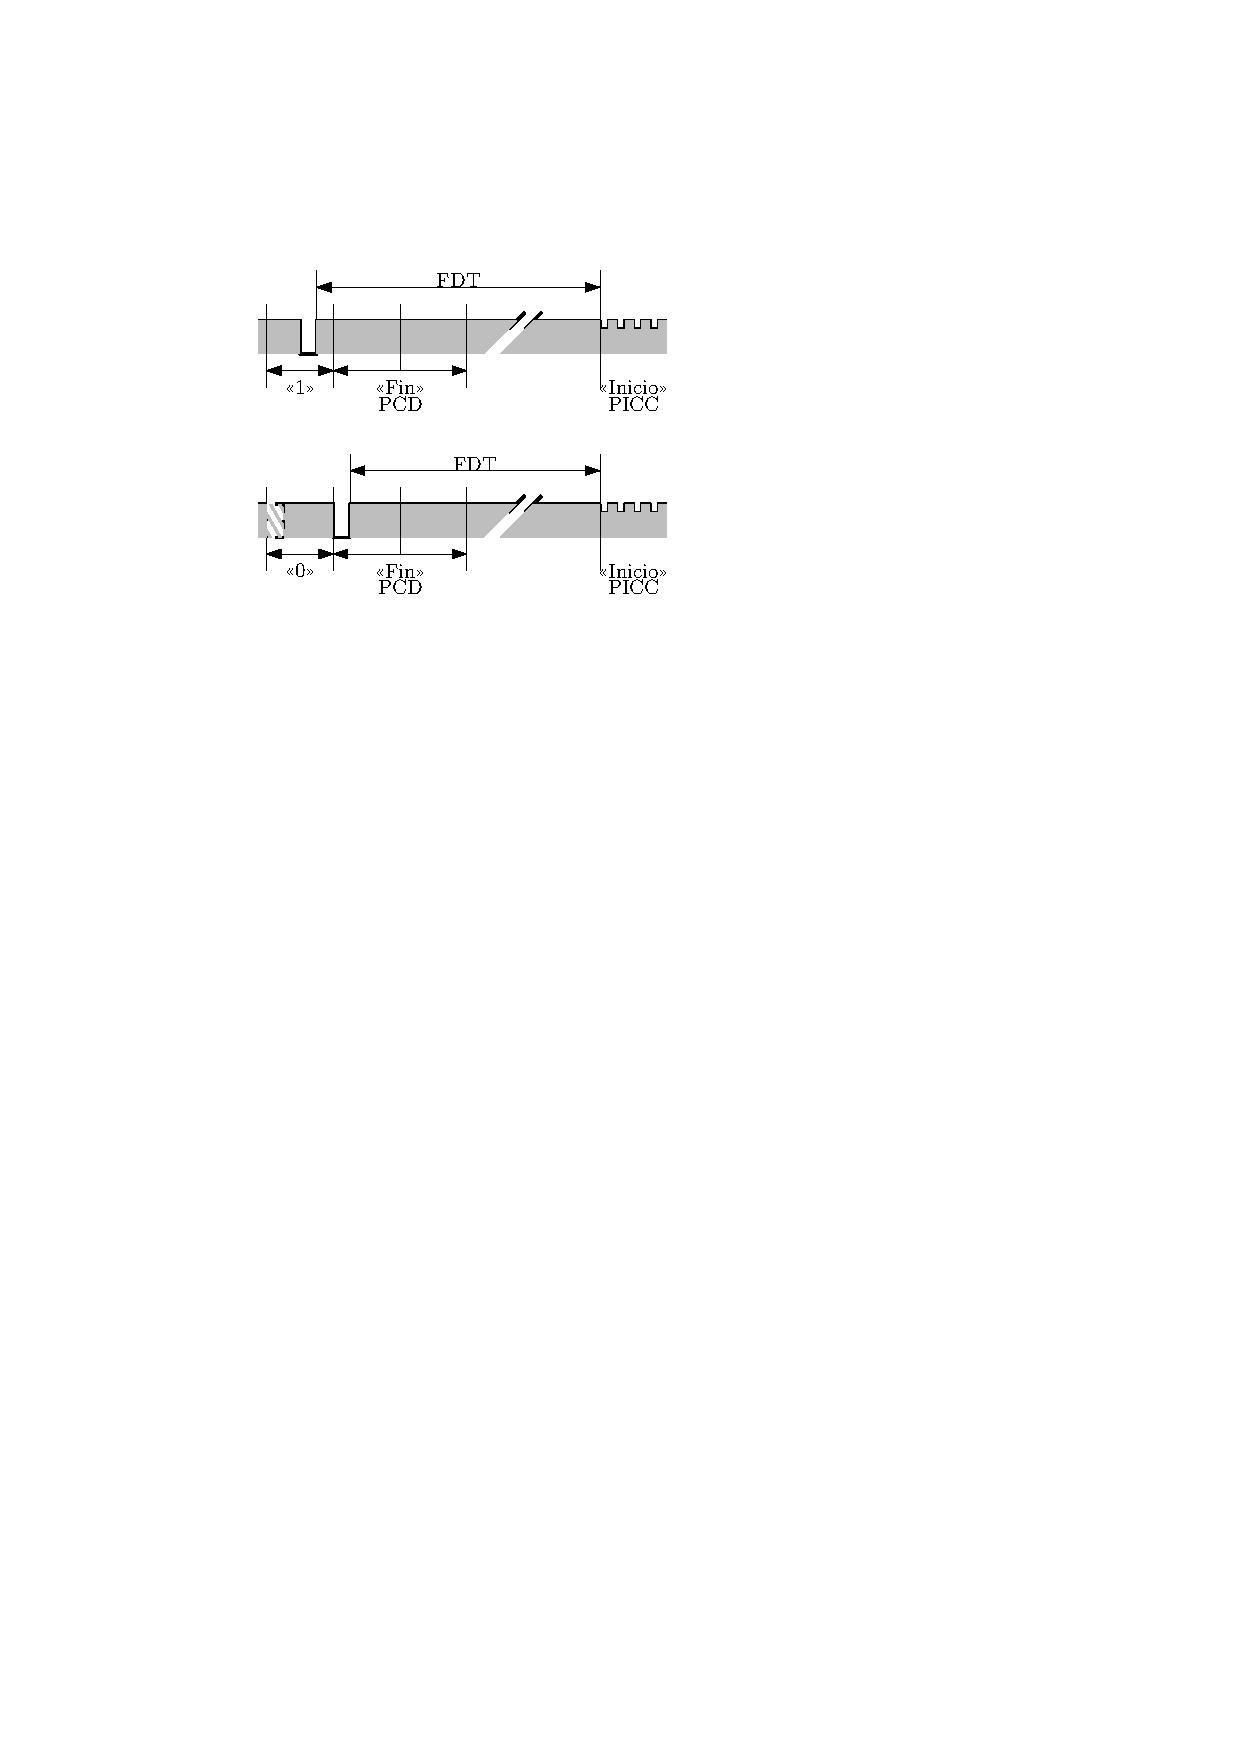
\includegraphics{EsquemaFDT_PCD_PICC}
	
	\caption{El tiempo de demora entre tramas (FDT: \emph{Frame Delay Time}) 
	de PCD a PICC depende del último bit de información transmitido.}
	
	\label{fig:EsquemaFDT_PCD_PICC}
\end{figure}

El <<FDT de PCD a PICC>> depende del último bit transmitido por el PCD, ya 
que de tratarse de un <<0>> lógico el símbolo de fin de comunicación estará 
representado por las secuencias Z e Y, mientras que si la transmisión del 
PCD finaliza con un <<1>> lógico el símbolo de <<Fin>> serán dos secuencias 
Y, según la codificación de la tabla \ref{tab:CodificacionPCD_PICC}. Esto 
cambia el instante en que se produce la última pausa, que es desde donde 
comienza a correr el tiempo de demora. El estándar define este tiempo como 
el correspondiente a \(N \cdot 128 + 84\) períodos de la señal portadora, 
cuando el último bit transmitido por el PCD es un <<1>>, y \(N \cdot 128 + 20
\) cuando el último bit es un <<0>>. \(N\) debe ser igual a 9 cuando se 
responde a los comandos de inicialización (REQA, WUPA, SELECT) dando como 
resultado 1236 o 1172 períodos respectivamente. Para cualquier otro comando 
\(N\) deberá ser mayor o igual a 9.

\bigskip
La tercera parte del estándar define tres tipos de tramas que son utilizadas 
en contextos particulares. Todas ellas comienzan con el símbolo <<Inicio>> 
de comunicación, finalizan con el símbolo <<Fin>> de comunicación y siempre 
los datos son enviados comenzando por el bit menos significativo. En la 
figura \ref{fig:TramasISO14443_3} se observa la estructura de este tipo de 
tramas. 

\begin{figure}
	\centering
	\begin{subfigure}{\textwidth}
		\centering
		
\includegraphics{TramaCortaISO14443_3}
		\caption{Trama corta: 7 bits que representan un comando y los 
			símbolos de <<Inicio>> y <<Fin>> de comunicación.}
		\label{fig:TramaCortaISO14443_3}
    \end{subfigure}%
    \vspace{5mm}
    \begin{subfigure}{\textwidth}
	    \centering
		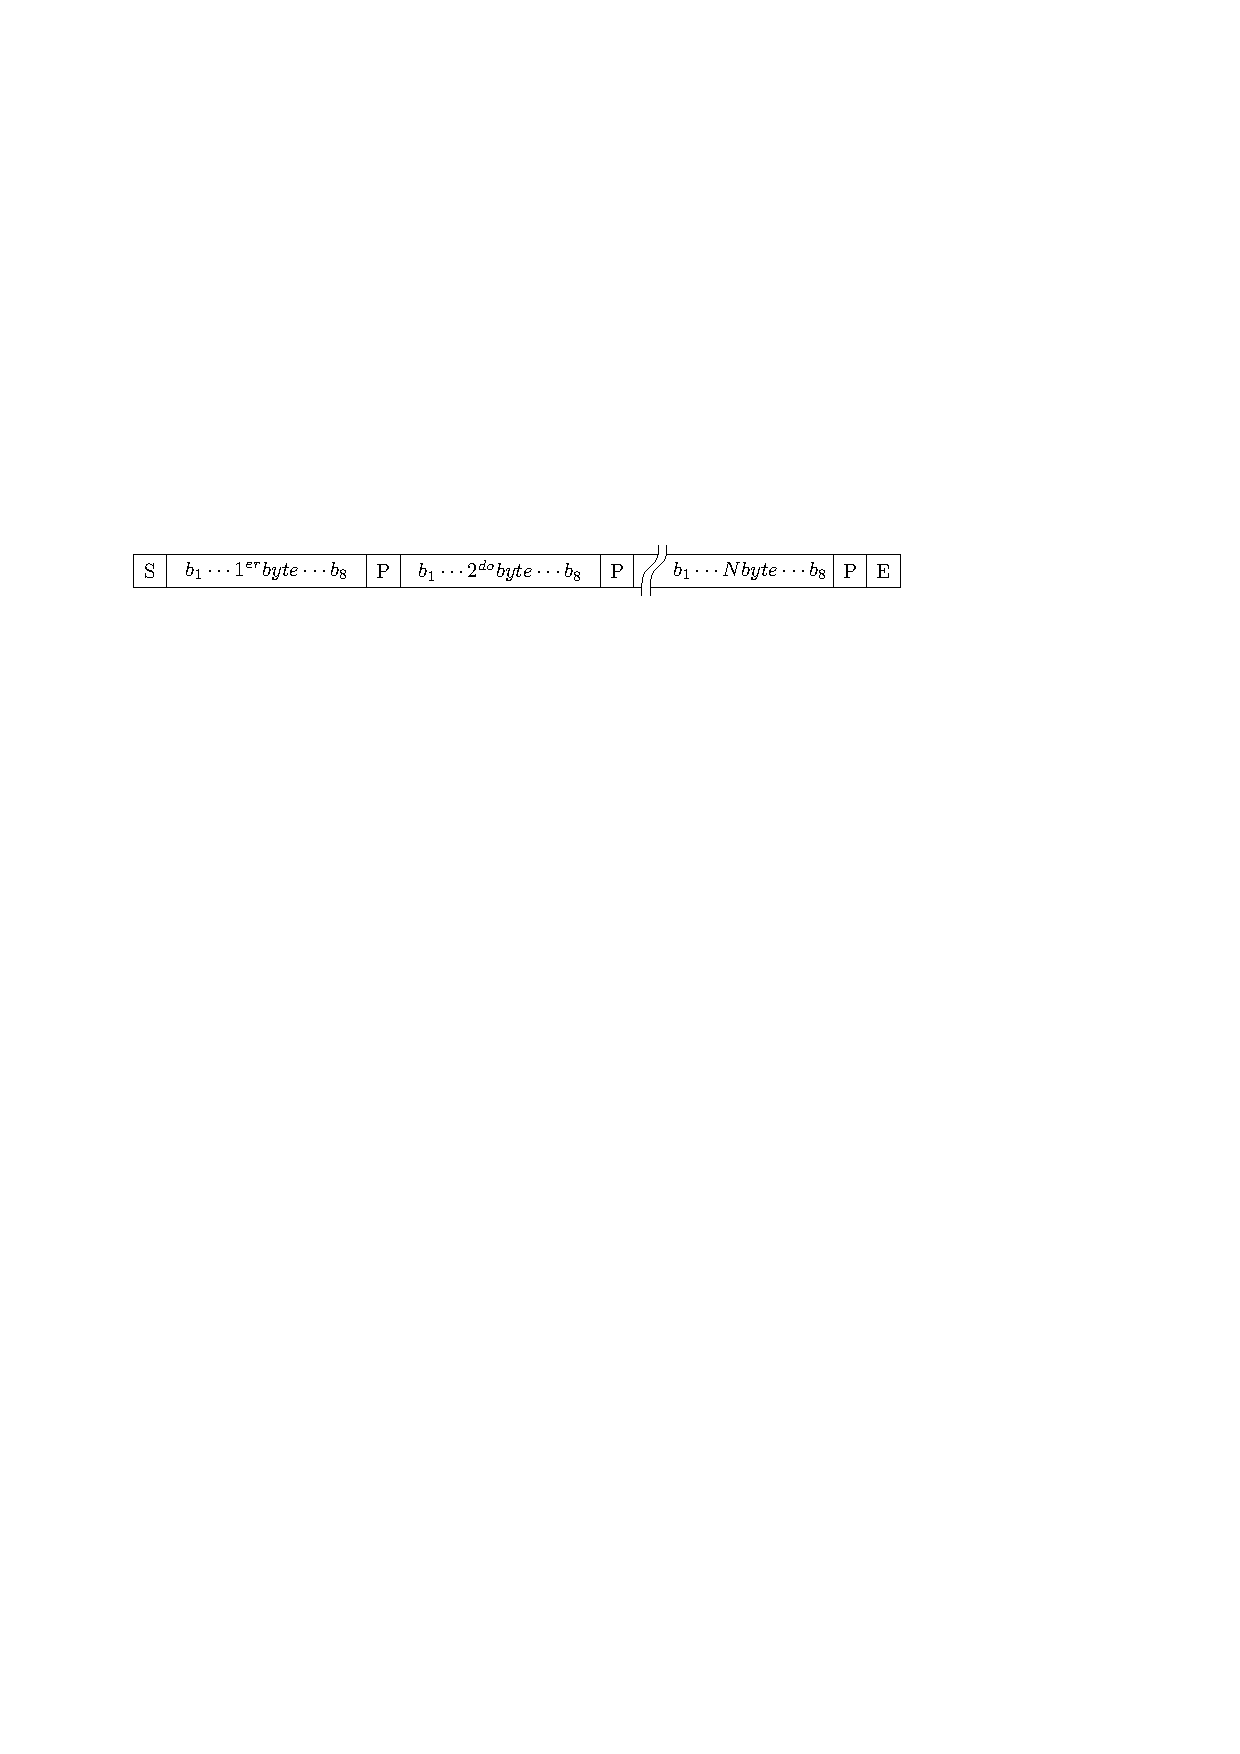
\includegraphics[width=\textwidth]{TramaEstandarISO14443_3}
		\caption{Trama estándar: N bytes, cada uno formando un dupla con el 
			bit de paridad de forma tal que la cantidad de <<1>> de la dupla sea 
			impar.}
		\label{fig:TramaEstandarISO14443_3}
    \end{subfigure}%
    \vspace{5mm}
    \begin{subfigure}{\textwidth}
		\centering
		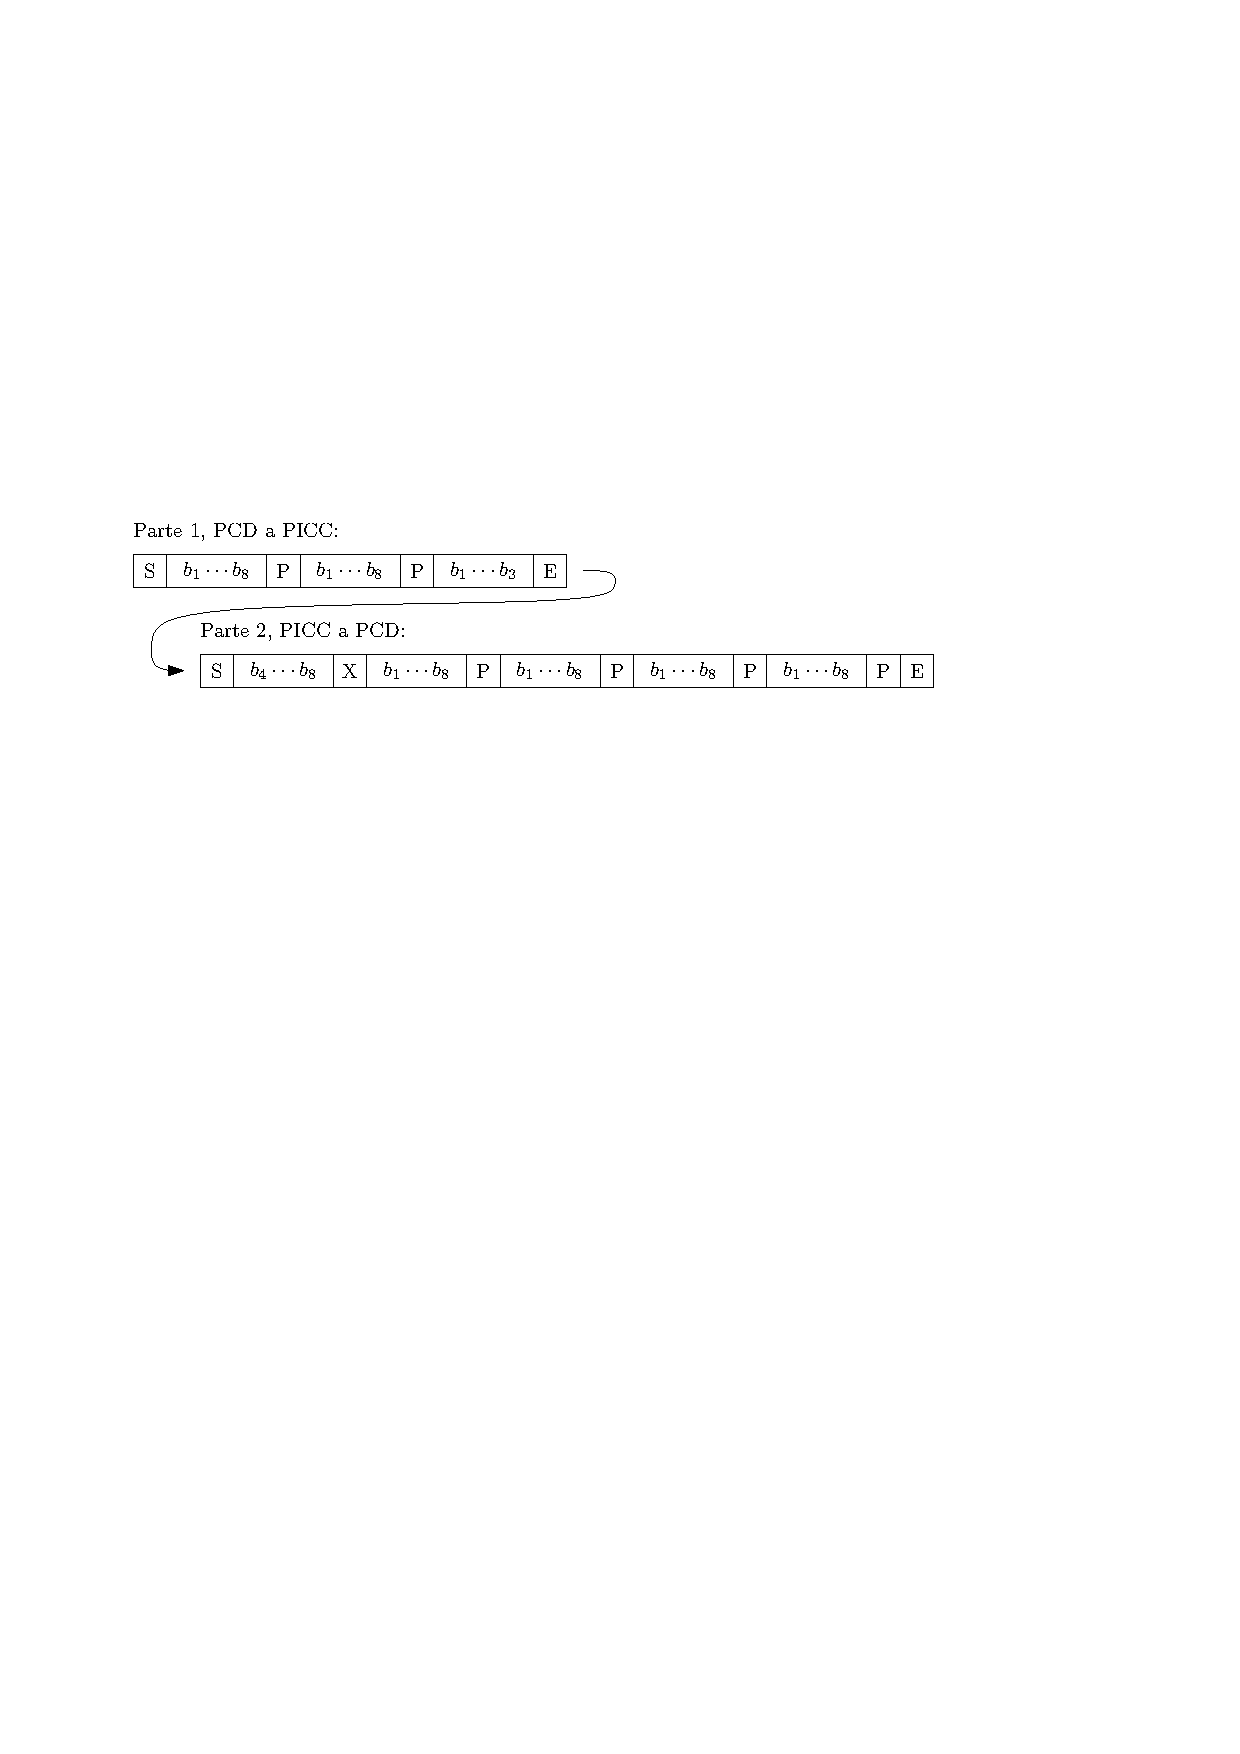
\includegraphics[width=\textwidth]{TramaAnticolISO14443_3}
		\caption{Trama anticolisión: Se divide la trama estándar en dos 
			partes. La división puede darse en cualquier lugar salvo en los dos 
			primeros bytes. El bit de paridad correspondiente al byte dividido 
			no se tiene en cuenta.}
		\label{fig:TramaAnticolISO14443_3}
    \end{subfigure}%
	\caption{Tramas definidas por el estándar.}
	\label{fig:TramasISO14443_3}
\end{figure}


La primer trama es llamada <<trama corta>> (\emph{short frame}) y es 
utilizada por el lector para iniciar la comunicación a través de comandos 
simples. Está compuesta por 7 bits que representan el comando que envía el 
PCD a la PICC.

Por otro lado se define la <<trama estándar>> (\emph{standard frame}) que se 
utiliza para el intercambio de información. Es un trama de longitud variable 
con N bytes (\(N \times 8\) bits) de datos, transmitidos en serie luego del 
símbolo de <<Inicio>>. A cada byte se le agrega un bit de paridad P de forma 
tal que la cantidad de unos lógicos por dupla (byte;P) sea impar. 

La tercera trama es llamada <<trama anticolisión orientada a bits>> (\emph
{Bit Oriented Anticollision Frame}). Se trata de una trama estándar de 7 
bytes de largo dividida en dos partes. La primer parte es enviada por el PCD 
a la PICC y contiene el comando de selección de tarjeta, la cantidad de bits 
válidos que serán transmitidos y parte del número de identificación (ID) de 
una de las PICC. El resto del número de identificación se completa con la 
respuesta de la PICC, que envía la segunda parte de la trama anticolisión 
sólo si el número de identificación parcial transmitido por el PCD coincide 
con el comienzo del ID de la tarjeta. En el caso en que el número de 
identificación parcial transmitido por el PCD coincida con parte del ID de 
más de una tarjeta, todas ellas responderán en forma sincronizada con la 
parte restante de su propio ID, produciéndose en ese caso colisiones en los 
bits que sean diferentes.

Se dice que hubo una colisión cuando dos transponders transmiten en forma 
sincronizada bits diferentes. Cuando esto ocurre se modula con la 
subportadora el tiempo completo de duración de un bit, ya que si, por 
ejemplo, una tarjeta transmite un <<1>> y la otra un <<0>>, la primera 
modula con subportadora durante una mitad del bit y la segunda modula la 
otra mitad del bit, dando como resultado una modulación completa. El lector 
debe ser capaz de detectar este tipo de colisiones.

\bigskip
Finalmente la tercera parte de la norma define una serie de estados que 
deben atravesar las PICC desde que reciben la alimentación hasta que una de 
ellas es seleccionada para establecer una comunicación. Al ingresar dentro 
del campo del PCD una tarjeta debe comenzar en el estado IDLE. En ese 
momento el lector puede realizar el intercambio de datos con otra PICC 
dentro del alcance sin ser interrumpido por la tarjeta que acaba de 
ingresar, ya que las PICC en el estado IDLE solo responderán a los comandos 
REQA (\emph{Request A}) o WUPA (\emph{Wake UP A}) \cite[sec.~6.4.1]
{ISO14443Part3}. Estos comandos son enviados por el PCD en forma de tramas 
cortas, lo que asegura que los datos destinados a otra PICC dentro de la 
zona de interrogación no sean falsamente interpretados como comandos REQA o 
WUPA.

Si una tarjeta en estado IDLE recibe un comando REQA válido deberá contestar 
con una trama estándar ATQA (\emph{Answer To Request A}) de dos bytes de 
longitud. Luego de enviar la respuesta la tarjeta pasa al estado READY. El 
lector reconoce entonces que existe al menos un transponder dentro del campo 
de interrogación y por lo tanto comienza el algoritmo anticolisión 
transmitiendo el comando SELECT \cite[sec.~6.4.2]{ISO14443Part3}.

El procedimiento anticolisión utilizado funciona como un algoritmo de 
búsqueda binaria. La primer parte de la trama anticolisión es utilizada para 
informar el criterio de búsqueda de un ID con un determinado número de bits 
válidos NVB (\emph{Number of Valid Bits}), mientras que la segunda parte 
contiene las respuestas de todas las PICC que cumplen con el criterio 
informado. Si se produce al menos una colisión en las respuestas, el PCD 
incrementa el número de bits validos decidiendo por una u otra de las PICC 
que produjeron la colisión. El algoritmo finaliza cuando no existen 
colisiones y el lector obtiene el ID completo de una de las tarjetas.

El largo de un número de identificación simple es de 4 bytes \cite
[sec.~6.5.4]{ISO14443Part3}. Para elegir una de las PICC el lector envía el 
comando SELECT seguido de \((4 \times 8)\) bits válidos. El transponder cuyo 
ID fue enviado debe confirmar el comando de selección respondiendo SAK (\emph
{Select AcKnowledge}) y pasar al estado ACTIVE. En este estado se realiza el 
intercambio de paquetes de datos, que se definen en la parte 4 de la norma y 
están fuera del alcance del presente trabajo.

Cuando el lector finaliza la comunicación con una PICC envía el comando HALT 
y pone al transponder en un estado de reposo similar a IDLE. En este estado 
el transponder solo responderá al comando WUPA, que se utiliza para volver 
poner el tag en el estado READY y volver a comenzar. En caso de existir un 
error en la comunicación el transponder debe pasar automáticamente al estado 
HALT.

\begin{figure}
	\centering
	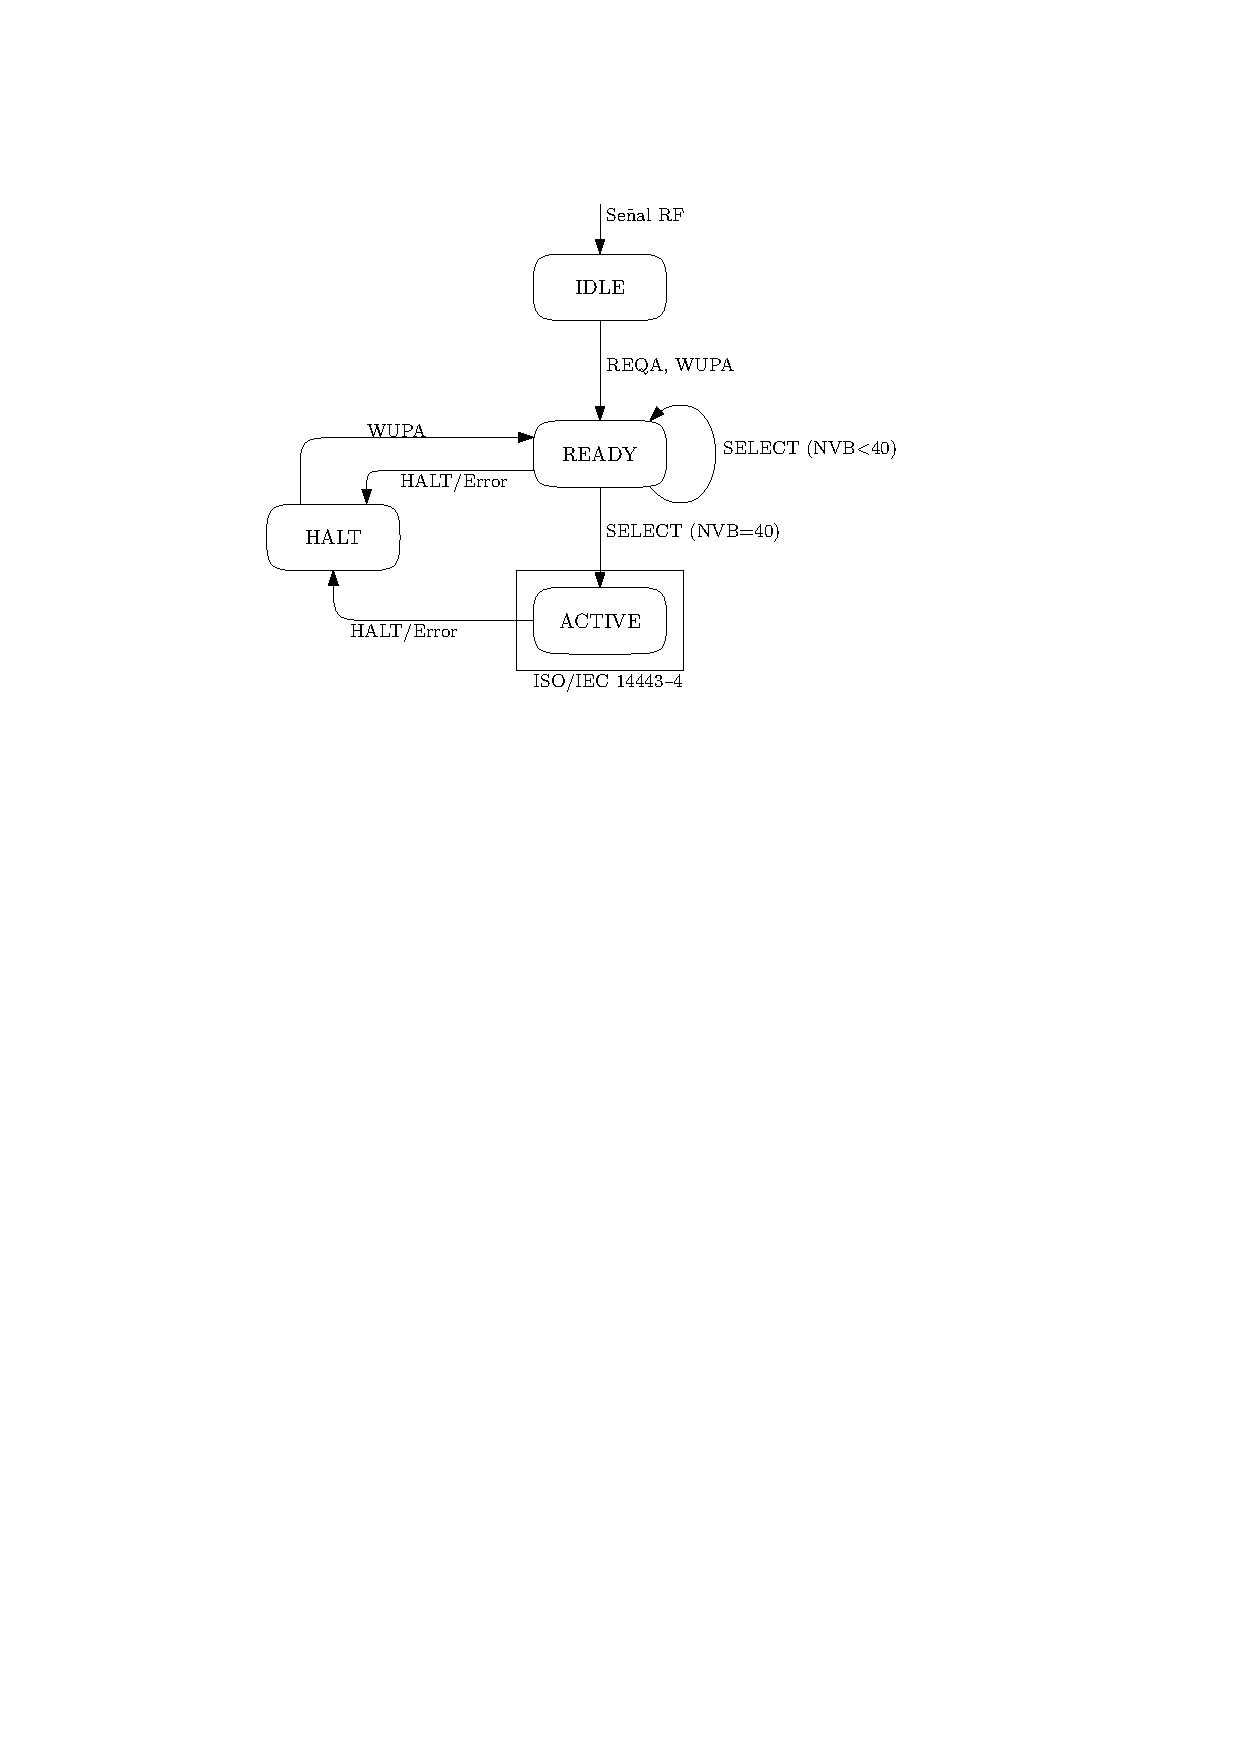
\includegraphics{MaquinaEstadosISO14443}
	\caption{Diagrama de estados del transponder de acuerdo al estándar 
		ISO/IEC 14443.}
	\label{fig:MaquinaEstadosISO14443}
\end{figure}

\section{Resumen del capítulo}

En este capítulo se presentó una breve introducción al tema de RFID, 
donde se explicó la teoría básica de funcionamiento, la transmisión 
de energía, de datos y reloj entre lector y transponder. Luego se hizo 
un repaso por los tipos de sistemas de RFID existentes y su 
clasificación y finalmente se llegó al estándar ISO/IEC 14443, que 
es la norma en que se basa el dispositivo a diseñar. A continuación 
se hará una pequeña reseña del capítulo que el lector debería tener 
presente a medida que avanza con la lectura:

\begin{itemize}
	\item Se llama PCD (\emph{Proximity Coupling Device}) al lector, 
	es decir, el dispositivo que produce el campo magnético, y 
	PICC (\emph{Proximity Integrated Circuit Card}) al transponder, el 
	dispositivo que contiene la información.
	
	\item En la norma se trabaja con acoplamiento inductivo a una 
	frecuencia \(f_{c}=\SI{13.56}{\mega\hertz}\). A esta señal se la 
	llama \emph{señal portadora}.
	
	\item El transponder debe funcionar dentro del rango de intensidad 
	de campo dado por la tabla \ref{tab:NivelesDeCampo}.
	
	\item La comunicación es del tipo pregunta-respuesta. El lector 
	mantiene el campo dentro de su volumen de operación y encuesta a los 
	transponders que ingresan dentro del volumen.
	
	\item El PCD transmite hacia la PICC modulando la portadora en ASK 
	100\% según las secuencias de la tabla 
	\ref{fig:SecuenciasPCD_PICC}.
	
	\item La PICC transmite hacia el PCD a través de modulación de 
	carga. La portadora es modulada con una subportadora de frecuencia 
	\(f_{s}=\sfrac{f_{c}}{16}\) según las secuencias de la tabla 
	\ref{tab:CodificacionPICC_PCD}. Existe una amplitud mínima de 
	modulación que debe superarse.
	
	\item El FDT (\emph{Frame Delay Time}) es el tiempo de demora 
	entre el fin de la transmisión del lector y el inicio de la 
	respuesta del transponder.
	
	\item Existen tres tipos de tramas: corta, estándar y 
	anti-colisión.
\end{itemize}
